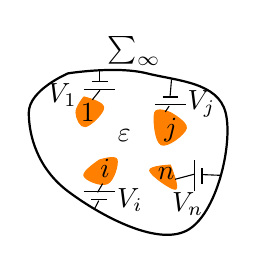
\begin{tikzpicture}

\draw [thick] plot[smooth, tension=.7] coordinates {(0,2.5) (-0.5,2) (0,1) (1.5,0.5) (2,2) (1,2.5) (0,2.5)};
\draw [orange, fill] plot[smooth, tension=.7] coordinates {(0.2,2.2) (0.1,2) (0.2208,1.8238) (0.4508,2.0688) (0.2,2.2)};
\draw [orange, fill]  plot[smooth, tension=.7] coordinates {(1.3,2) (1.1,2) (1.1808,1.5938) (1.5,1.8) (1.3,2)};
\draw  [orange, fill] plot[smooth, tension=.7] coordinates {(0.4,1.4) (0.2,1.2) (0.5,1.1) (0.62,1.405) (0.4,1.4)};
\draw [orange, fill]  plot[smooth, tension=.7] coordinates {(1.2958,1.3338) (1.0358,1.2638) (1.3658,1.0288) (1.2958,1.3388)};
\node at (0.2508,1.9988) {$1$};
\node at (1.3058,1.7738) {$j$};
\node at (0.4708,1.2988) {$i$};
\node at (1.2458,1.2238) {$n$};
\draw (0.2,2.3) -- (0.6,2.3);
\draw (0.3,2.4) -- (0.5,2.4);
\draw (1.1,2.1) -- (1.5,2.1);
\draw (1.2,2.2) -- (1.4,2.2);
\draw (0.1958,0.9938) -- (0.5958,0.9938);
\draw (0.2958,0.8938) -- (0.4958,0.8938);
\draw (1.6,1) -- (1.6,1.4);
\draw (1.7,1.1) -- (1.7,1.3);
\draw (1.3579,1.1544) -- (1.6029,1.2194);
\draw (1.6979,1.2144) -- (1.9429,1.2044);
\draw (0.4379,1.0994) -- (0.3737,0.9882);
\draw (0.3887,0.8832) -- (0.3329,0.7744);
\draw (0.4029,2.5244) -- (0.4029,2.3894);
\draw (0.4029,2.2844) -- (0.3079,2.1644);
\draw (1.3129,2.4244) -- (1.2929,2.1894);
\draw (1.2829,2.0844) -- (1.2329,2.0094);
\node at (-0.0721,2.2194) {$V_1$};
\node at (1.6929,2.1144) {$V_j$};
\node at (0.7829,0.8944) {$V_i$};
\node at (1.5179,0.8444) {$V_n$};
\node at (0.7129,1.7094) {$\varepsilon$};
\node at (0.8379,2.7783) {$\sum_\infty$};
\end{tikzpicture}